\documentclass[aps,pre,twocolumn,showpacs,preprintnumbers,amsmath,amssymb]{revtex4-1}
%\documentclass[preprint,showpacs,preprintnumbers,amsmath,amssymb]{revtex4}

% Some other (several out of many) possibilities
%\documentclass[preprint,aps]{revtex4}
%\documentclass[preprint,aps,draft]{revtex4}
%\documentclass[prb]{revtex4}% Physical Review B

\usepackage{graphicx}% Include figure files
\usepackage{dcolumn}% Align table columns on decimal point
\usepackage{bm}% bold math 

\usepackage[latin1]{inputenc}
\usepackage{amsfonts}
\usepackage{amsmath}
\usepackage{amssymb}
\usepackage{amsthm}
\usepackage{bbold}
\usepackage{color}
\usepackage[american]{babel}
\usepackage[T1]{fontenc}
\usepackage{longtable}
%\usepackage[dvips]{graphicx}
\usepackage{xspace}
\usepackage{bbm}
\usepackage[all]{xy}
%\usepackage{slashbox}
%\usepackage[justification=centering]{caption}
\providecommand{\begeq}[1]{\begin{equation}#1\end{equation}}
\DeclareMathOperator{\tr}{tr}
\providecommand{\norm}[1]{\lVert#1\rVert}
\newtheorem{theorem}{Theorem}
\newtheorem{lemma}{Lemma}
\newtheorem{defi}{Definition}
\newtheorem{rem}{Remark}
\newtheorem{conj}{Conjecture}
\newtheorem{prop}{Proposition}
\DeclareMathOperator{\con}{cond}
\DeclareMathOperator{\diag}{diag}
\newcolumntype{C}[1]{>{\centering\arraybackslash}p{#1}}

\begin{document}

%\preprint{APS/123-QED}

\title{TBD}% Force line breaks with \\

%\author{}
%\author{}
%\affiliation{
%}
%Lines break automatically or can be forced with \\

\author{Varadarajan Rengaraj}
\email{rengaraj@campus.uni-paderborn.de}
%\affiliation{Institute for Physical Chemistry and Center for Computational Sciences, Johannes Gutenberg University of Mainz, Staudinger Weg 7, D-55128 Mainz, Germany}
%\affiliation{
%Dynamics of Condensed Matter and Center for Sustainable Systems Design, Department of Chemistry, University of Paderborn, Warburger Str. 100, D-33098 Paderborn, Germany
%}
\affiliation{Department of Computer science, Paderborn University, Warburger Str. 100, D-33098 Paderborn, Germany}

\author{Michael Lass}
\email{michael.lass@uni-paderborn.de}
%\affiliation{Institute for Physical Chemistry and Center for Computational Sciences, Johannes Gutenberg University of Mainz, Staudinger Weg 7, D-55128 Mainz, Germany}
%\affiliation{
%Dynamics of Condensed Matter and Center for Sustainable Systems Design, Department of Chemistry, University of Paderborn, Warburger Str. 100, D-33098 Paderborn, Germany
%}
\affiliation{Department of Computer science, Paderborn University, Warburger Str. 100, D-33098 Paderborn, Germany}

\author{Christian Plessl}
\email{christian.plessl@uni-paderborn.de}
%\affiliation{Institute for Physical Chemistry and Center for Computational Sciences, Johannes Gutenberg University of Mainz, Staudinger Weg 7, D-55128 Mainz, Germany}
%\affiliation{
%Dynamics of Condensed Matter and Center for Sustainable Systems Design, Department of Chemistry, University of Paderborn, Warburger Str. 100, D-33098 Paderborn, Germany
%}
\affiliation{Department of Computer science, Paderborn University, Warburger Str. 100, D-33098 Paderborn, Germany}

\author{Thomas D. K\"uhne}
\email{tdkuehne@mail.upb.de}
%\affiliation{Institute for Physical Chemistry and Center for Computational Sciences, Johannes Gutenberg University of Mainz, Staudinger Weg 7, D-55128 Mainz, Germany}
%\affiliation{%
%Dynamics of Condensed Matter and Center for Sustainable Systems Design, Department of Chemistry, University of Paderborn, Warburger Str. 100, D-33098 Paderborn, Germany
%}
\affiliation{Department of Chemistry, Paderborn University, Warburger Str. 100, D-33098 Paderborn, Germany}

\date{\today}% It is always \today, today,
             %  but any date may be explicitly specified


\begin{abstract}

\end{abstract}

%A Valid PACS numbers may be entered using the \verb+\pacs{#1}+ command.
\pacs{31.15.-p, 31.15.Ew, 71.15.-m, 71.15.Pd}% PACS, the Physics and Astronomy
                             % Classification Scheme.
\keywords{}%Use showkeys class option if keyword
                              %display desired
\maketitle



\section{Introduction}
Molecular dynamics (MD) is a standard technique to study the movement of atoms in a substance over time. It involves computing the forces on all atoms for every time step as a product of the bonded and non- bonded interactions. This is done by numerically solving the Newton's law of motions and update the parameters such as velocity and position of each atom. Computing the forces from non-bonded interactions is computationally expensive and our conventional multicore processors falls behind on the computational requirements. There has been numerous efforts going in this area to accelerate the MD simulations especially the ones based on graphics processing unit (GPU) and field-programmable gate array (FPGA).   
Microchips sizes of FPGA and GPU, are on a constant decline to accommodate more transistors but it also makes the transistors susceptible to both temporary and permanent failures. These hardware faults occasionally propagate to the software and considering this aspect, there is a renewed interest in approximate computing that can be applied in the software to give us the outputs that does not diverge too much from the ideal outputs. Approximate computing also ensures that the portion of investment needed in detecting the hardware faults, avoidance and recovery is avoided. The research goal of approximate computing is to explore techniques to gain more efficiency by relaxing the exactness of calculated outputs compared to the ideal outputs. In this paper, we describe one such technique that relaxes the exactness of the output and we explore to what extent it diverges from the ideal output.


\section{Methodology}
To demonstrate approximate computing, we introduce a computational error, a statistical noise to the forces computed on the atom when running the MD simulation. In this section, we describe in detail on how we introduce the computational error, a process we mimic in our standard system instead of running the MD on the actual FPGA or GPU hardware. We classify the computational errors into two types 1. Fixed point error 2. Floating point error. 
Fixed point error is described by the following equation. 
\begin{equation}
\begin{pmatrix}
\textbf{F}_{I}^{FPGA(x)}\\ 
\textbf{F}_{I}^{FPGA(y)}\\ 
\textbf{F}_{I}^{FPGA(z)}\\ 

\end{pmatrix} = 
\begin{pmatrix}
\textbf{F}_{I}^{x}\\ 
\textbf{F}_{I}^{y}\\ 
\textbf{F}_{I}^{z}\\ 

\end{pmatrix} + 
\begin{pmatrix}
c_{1}.10^{-\beta }\\ 
c_{2}.10^{-\beta }\\ 
c_{3}.10^{-\beta }\\ 

\end{pmatrix}
\end{equation}
 
Floating point error is described by the following equation.
\begin{equation}
\begin{pmatrix}
\textbf{F}_{I}^{FPGA(x)}\\ 
\textbf{F}_{I}^{FPGA(y)}\\ 
\textbf{F}_{I}^{FPGA(z)}\\ 

\end{pmatrix} = 
\begin{pmatrix}
\textbf{F}_{I}^{x}.10^{-\alpha1}\\ 
\textbf{F}_{I}^{y}.10^{-\alpha2}\\ 
\textbf{F}_{I}^{z}.10^{-\alpha3}\\ 

\end{pmatrix} + 
\begin{pmatrix}
c_{1}.10^{-(\alpha1+\beta)}\\ 
c_{2}.10^{-(\alpha2+\beta)}\\ 
c_{3}.10^{-(\alpha3+\beta)}\\ 

\end{pmatrix}
\end{equation}

where c1, c2 and c3 are random values chosen in the range [-0.5, 0.5]. The values of \(\beta\) that were used in our simulation runs are discussed in detail in the computational details section. \(\textbf{F}_{I}\) is the exact consistent force and \(\textbf{F}_{I}^{FPGA}\) is the force computed when MD is run on the FPGA.

We use Langevin equations in molecular dynamics for the purpose of demonstrating that the computational errors introduced by the methods described above can be effectively compensated by an existing framework. 
For the langevin dynamics (LD) run on a FPGA or GPU based accelerators, we assume at this point a computational error \(\mathbf{\Xi }_{I}^{N}\) is added to the force that is computed and the force that we get at the output is not the exact force \(\textbf{F}_{I}\) but an approximation
\begin{equation}
\textbf{F}_{I}^{FPGA} = \textbf{F}_{I}+ \mathbf{\Xi }_{I}^{N}
\end{equation} 
Fortunately in our case, it is still possible to accurately obtain Boltzmann sampling by means of a modified Langevin equation 
\begin{equation}
M_{I}\ddot{\textbf{R}}_{I}=\textbf{F}_{I}+\mathbf{\Xi }_{I}^{N}-\gamma _{N}M_{I}\dot{\textbf{R}}_{I} 
\end{equation}
which in our case is,
\begin{equation}
M_{I}\ddot{\textbf{R}}_{I} = \textbf{F}_{I}^{FPGA}-\gamma _{N}M_{I}\dot{\textbf{R}}_{I}
\end{equation}

where \(\textbf{R}_{I}\) are the positions of the atoms, \(M_{I}\) the corresponding atomic nuclear masses and \(\gamma _{N}\) is a friction coefficient which is approximately chosen to compensate for the additive white noise \(\mathbf{\Xi }_{I}^{N}\) which in this case is unbiased.
The additive white noise therefore has to obey

\begin{equation}
 \left \langle \textbf{F}_{I}\left ( 0 \right ) \mathbf{\Xi } _{I}^{N}\left ( t \right )\right \rangle \cong  0,
\end{equation}

and as well as the fluctuation-dissipation theorem

\begin{equation}
\left \langle \mathbf{\Xi } _{I}^{N}\left ( 0 \right ) \mathbf{\Xi } _{I}^{N}\left ( t \right ) \right \rangle \cong  2k_{B}TM\gamma _{I}^{N}\delta \left ( t \right )
\end{equation}  

We further present in this paper the method to effectively compensate for the additive noise introduced on the force using the existing langevin dynamics framework. 

 
\section{Computational details}

To demonstrate our method as described above, we have implemented it in the Frontiers in simulation technology (force field implementation) code which is part of the publicly available suite of programs CP2k \cite{cp2kwebsite}. We configured to run the langevin dynamics for the Silicon (Si) atom with a time step of 1 femtosecond (fs) at a temperature of 3000 K. The Empirical Interatomic Potential (EIP) calculation model for our MD simulation is Bazant potentials. The total number of Si atoms used for the MD simulation is thousand with a cubic cell length of 27.155 Angstrom. 

Langevin dynamics configured for the above settings have been run with frictional coefficient \(\gamma\) assigned a value equal to 1/1000 \(fs^{-1}\). This simulation run is considered as the reference with which the computational error introduced simulations are compared. As described in the Methodology section, computational errors are classified as fixed point error and floating point error. With necessary changes incorporated to the cp2k software, two different builds for the two variants of errors have been made and Langevin dynamics were performed on those builds. Three different cases of fixed point errors were tested and for the equation representing fixed point error, the corresponding \(\beta\) value that was used were 1, 2 and 3. Similarly three different cases of floating point errors were tested and for the equation representing floating point error, the corresponding \(\beta\) value that was used were 0, 1, 2.

As discussed earlier in the methodology section, a separate frictional coefficient is necessary to compensate for the computational error that was  introduced in the builds. This frictional coefficient is managed through the parameter called shadow \(\gamma\) and this parameter is available in the langevin section of the cp2k software.   

The following tables lists down shadow \(\gamma\) values used for fixed point and floating point errors.  Units for \(\gamma\) and shadow \(\gamma\) is \(fs^{-1}\). As described in this paper \cite{ShadowGammaEstimate} an approximate value of shadow \(\gamma\) can be computed by integrating the autocorrelation function of the additive white noise. \\\\\\


\textbf{Table 1.} Shown are the shadow \(\gamma\) values for fixed point errors. \\ \\
\begin{table}[h!]
\begin{tabular}{|l|l|}
\hline
\textit{\(\beta\) } & \textit{Shadow \(\gamma\)} \\ \hline
1             & 0.0004                \\ \hline
2             & 0.000009              \\ \hline
3             & 0.0000009             \\ \hline
\end{tabular}
\end{table}


\textbf{Table 2.} Shown are the shadow \(\gamma\) values for floating point errors.\\

\begin{table}[h!]
\begin{tabular}{|l|l|}
\hline
\textit{\(\beta\) } & \textit{Shadow \(\gamma\)} \\ \hline
0             & 0.00025               \\ \hline
1             & 0.000005              \\ \hline
2             & 0.000005              \\ \hline
\end{tabular}
\end{table}
 
\section{Results and Discussion}

 In Fig. 1 and Fig. 2 we compare the pair correlation functions g(r) calculated with noisy forces and those evaluated with the standard approach. In Fig. 1 we show the pair correlation functions g(r) calculated with noisy forces generated from fixed point errors. In Fig. 2 we show the pair correlation functions g(r) calculated with noisy forces generated with floating point errors. We see from both Fig. 1 and Fig. 2, that the results are in agreement with our reference calculations and the use of noisy forces does not degrade the local structure and dynamics of the standard system. 

\begin{figure}[h!]%[!htpb,floatfix]
\begin{center}
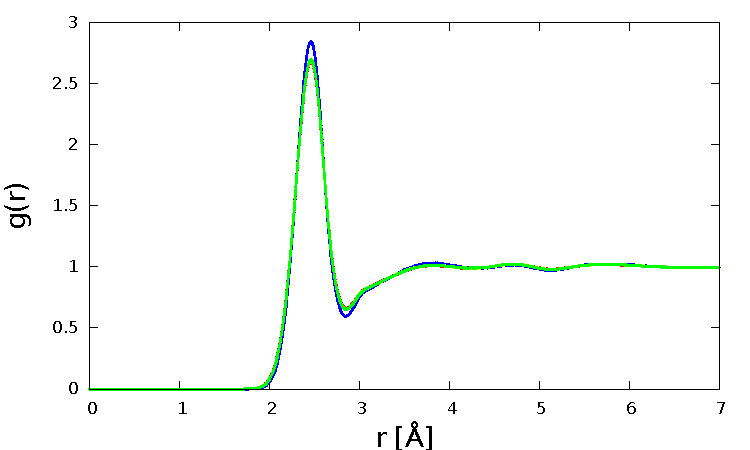
\includegraphics[width=0.475\textwidth]
{figures/fixedpoint.pdf}
\end{center}
\caption{\label{Fig1}
Pair correlation function for (a) liquid silicon (3000~K) in red and (b) liquid silicon (3000~K) with noisy forces introduced by fixed point errors corresponding to the values \(\left ( c.10^{-1 }\right ) \)(blue), \(\left ( c.10^{-2 }\right ) \)(yellow) and \(\left ( c.10^{-3 } \right ) \)(green).
} \end{figure}

\begin{figure}[h!]%[!htpb,floatfix]
\begin{center}
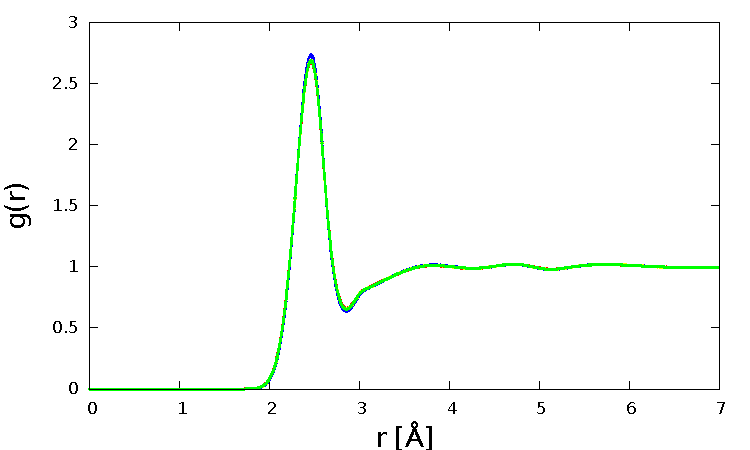
\includegraphics[width=0.475\textwidth]
{figures/floatingpoint.pdf}
\end{center}
\caption{\label{Fig2}
Pair correlation function for (a) liquid silicon (3000~K) in red and (b) liquid silicon (3000~K) with noisy forces introduced by floating point errors corresponding to the values \(c.10^{-(\alpha)}\)(blue), \(c.10^{-(\alpha+1)}\)(yellow) and \(c.10^{-(\alpha+2)}\)(green).
} \end{figure}

\begin{figure}[h!]%[!htpb,floatfix]
\begin{center}
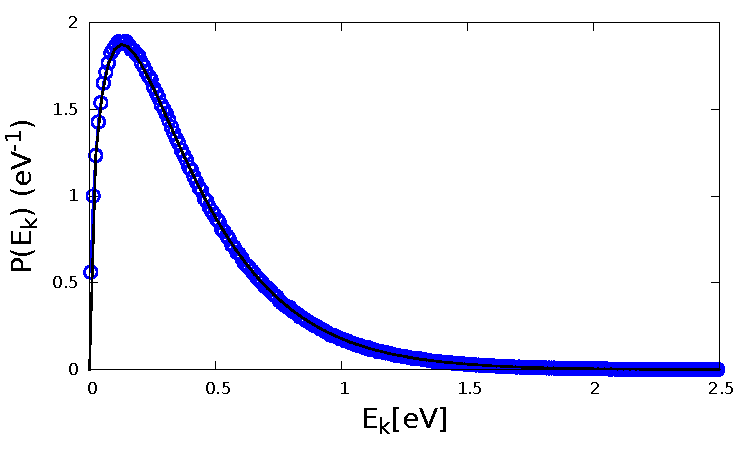
\includegraphics[width=0.475\textwidth]
{figures/maxwelldistribution.pdf}
\end{center}
\caption{\label{Fig3}
Statistical properties in a 1000 atoms liquid Si simulation at 3000~K. (a) The ionic kinetic energy distributions (line) is compared with the exact Maxwell distribution (circles).
} \end{figure}

In Fig. 3, the ionic kinetic energy distribution calculated with noisy forces is compared with the exact Maxwell distribution line and it can be seen that not only the average energy is correct but also its fluctuations follow the Maxwell distribution. 

\begin{figure}[h!]%[!htpb,floatfix]
\begin{center}
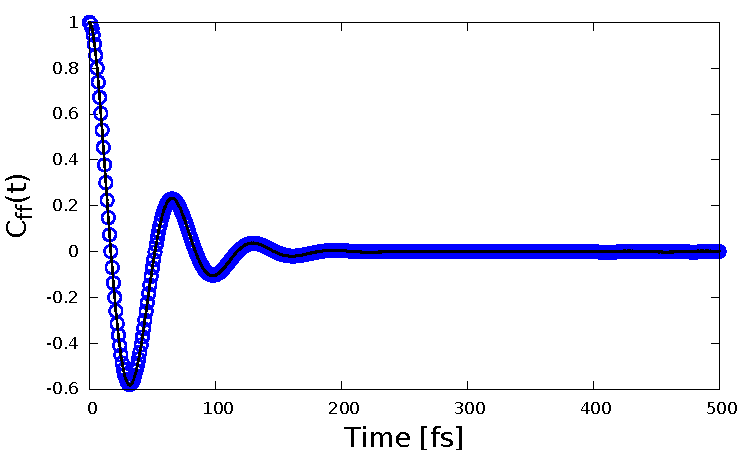
\includegraphics[width=0.475\textwidth]
{figures/force_autocorrelation.pdf}
\end{center}
\caption{\label{Fig4}
The Autocorrelation of the noisy force \(
 \left \langle \textbf{F}_{I}^{FPGA}\left ( 0 \right ) \textbf{F}_{I}^{FPGA}\left ( t \right )\right \rangle \)(line) is compared with the autocorrelation of the exact force \( \left \langle \textbf{F}_{I}\left ( 0 \right ) \textbf{F}_{I}\left ( t \right )\right \rangle \)(circles). 
} \end{figure}

The autocorrelation of the noisy force is expanded by the following equation, 

\begin{subequations}
\begin{equation}
\begin{split}
\left \langle \textbf{F}_{I}^{FPGA}\left ( 0 \right )\textbf{F}_{I}^{FPGA}\left ( t \right )\right \rangle = \linebreak \\ \left \langle \left ( \textbf{F}_{I}\left ( 0 \right ) + \mathbf{\Xi } _{I}^{N}\left(0 \right )\right) \left( \textbf{F}_{I}\left ( t \right )+\mathbf{\Xi } _{I}^{N}\left ( t \right )\right) \right \rangle
\end{split}
\end{equation}

\begin{equation}\label{eq:1}
\begin{split}
\left \langle \textbf{F}_{I}^{FPGA}\left ( 0 \right )\textbf{F}_{I}^{FPGA}\left ( t \right )\right \rangle = \left \langle \textbf{F}_{I}\left ( 0 \right ) \textbf{F}_{I}\left ( t \right )\right \rangle + \linebreak \\\left \langle \textbf{F}_{I}\left ( 0 \right ) \mathbf{\Xi } _{I}^{N}\left(t \right )\right \rangle +  \left \langle \textbf{F}_{I}\left ( t \right ) \mathbf{\Xi } _{I}^{N}\left(0 \right )\right \rangle + \left \langle \mathbf{\Xi } _{I}^{N}\left(0 \right ) \mathbf{\Xi } _{I}^{N}\left(t \right )\right \rangle
\end{split}
\end{equation}
\end{subequations}

In Eq. (\ref{eq:1}), the cross correlation terms between exact force and the additive white noise becomes zero, thereby giving us an equation where the autocorrelation of noisy force is equal to the autocorrelation of the exact force. From Fig. 4, we prove this behavior where the autocorrelation of the noisy force is compared with the autocorrelation of the exact force. 

If the random value that was used to generate the computational error is chosen in the range [0,1] instead of [-0.5,0.5], we encounter a phenomenon called "Flying Ice Cube" \cite{flyingIceCube} during our MD simulations.  


\section{Summary}

To summarize, in this paper, we described the method to compensate for the computational errors that are introduced when running the MD code in FPGA or GPU using approximate computing technique.  


\begin{acknowledgments}
The authors would like to thank the Gauss Center for Supercomputing (GCS) for providing computing time through the John von Neumann Institute for Computing (NIC) on the GCS share of the supercomputer JUQUEEN at the J\"ulich Supercomputing Centre (JSC). This project has received funding from the European Research Council (ERC) under the European Union's Horizon 2020 research and innovation programme (grant agreement No 716142).
\end{acknowledgments}

%\bibliography{paper}

\begin{thebibliography}{10}

%\bibitem{ball}
%P.~Ball,
%\newblock {\em Life's Matrix: A Biography of Water}
%\newblock (Univ of California Press 2001).
\bibitem{cp2kwebsite} 
CP2K Open Source Molecular Dynamics,
\\\texttt{http://cp2k.berlios.de}

\bibitem{bazantEIP} 
EIP Bazant potential,
\textit{tofill}

\bibitem{ShadowGammaEstimate} 
Khaliullin, Rustam Z, VandeVondele, Joost, Hutter, Juerg. 
\textit{Efficient Linear-Scaling Density Functional Theory for Molecular Systems}

\bibitem{flyingIceCube} 
Stephen C. Harvey, Robert K.-Z. TAN, Thomas Cheatham. 
\textit{The Flying Ice Cube: Velocity Rescaling in Molecular Dynamics Leads to Violation of Energy Equipartition}

\bibitem{NumericalStabilityQC} 
Gerald Knizia, Wenbin Li, Sven Simon, Hans-Joachim Werner. 
\textit{Determining the Numerical Stability of Quantum Chemistry Algorithms}


\end{thebibliography}

%-----

\end{document}

